\section{用户兴趣表示与匹配的研究}
本章将从用户兴趣的特征作为切入点,对每种特征进行深入分析,提出一套完整的兴趣表示方法。根据第二章中的讨论,兴趣具有最明显的两个特征是关联性和动态性。前者说明的是兴趣概念的关系如同名词之间的关系一样具有同义词、上义词和下义词等,文中提出了一种静态兴趣分类树的模型来充分表示这个特征。后者说明的是用户兴趣会随时间变化而变换,并且分为长期兴趣和短期兴趣,所以文中提出了一种动态兴趣伸展树的模型来解决这一变化的过程。此外,为了使系统能够自动地学习用户的兴趣爱好,以便将来可以为用户推荐兴趣(主题)相似的资源,文中提出了一种学习和推荐的方法来完成这个工作。

\subsection{基于文本主题的兴趣点描述方法}
在正式讨论兴趣树的细节之前,先对文本中涉及兴趣相关的概念进行说明和形式化定义。

给定大小为$V$的词汇表$\mathcal{V}=\{v_1,...,v_V\}$,对于大小为$K$的兴趣全集$\mathcal{I}=\{\vec{in}_1,...,\vec{in}_K\}$,其中$\vec{in}_i~(i\in [1,K])$为第$i$个兴趣点。在本文中,兴趣点的名称$name(\vec{in})$是一个字符串,兴趣点的值$value(\vec{in})$看做是从兴趣变量$\vec{x}$抽样出的一个观测值,兴趣变量$\vec{x}$服从Dirichlet分布,即:
\begin{equation*}
  p(\vec{x}|\vec{\alpha})=Dir(\vec{x}|\vec{\alpha})=\frac{\prod_{i=1}^{V}\Gamma(\alpha_i)}{\Gamma(\sum_{i=1}^{V}\alpha_i)}\cdot \sum_{i=1}^{V}x_i^{\alpha_i-1},~~(\vec{\alpha}=(\alpha_1,...,\alpha_V))
\end{equation*}
可以看出,兴趣点$\vec{in}$是一个$V$维的向量,向量中每个值表示当前词汇对兴趣的权重。因此,对于两个兴趣点$\vec{in}_i$和$\vec{in}_j$\$,它们之间的相似度$d_{i,j}$可以用余弦相似度来衡量:
\begin{equation}
  \label{eq:intsim}
  d_{i,j}=cos(\vec{in}_i,\vec{in}_j)
\end{equation}

要说明的是,这里的兴趣点的表示方式本质上是继承自文本中的主题,在下文没有特别说明的情况下,可以认为兴趣点等价于主题。同时,关于如何估计兴趣变量$\vec{x}$参数的方法就等同于如何在给定的语料库中训练出主题分布$\Phi$。所以,在这一章中,可以默认提取兴趣点的方式都已经存在,重点是如何利用这些兴趣点构建用户的兴趣树。

\subsection{静态兴趣分类树的表示方法}
这一节主要针对兴趣间的关联性问题,对整个兴趣集建立一个描述模型,从而能够展现出兴趣间的关系。从兴趣点的名称来看,这些名称一般为名词,自然而然地想到了兴趣点之间应该是一种层次关系,于是本节提出了用静态兴趣分类树的方式进行描述整个兴趣集。

\begin{figure}
\centering
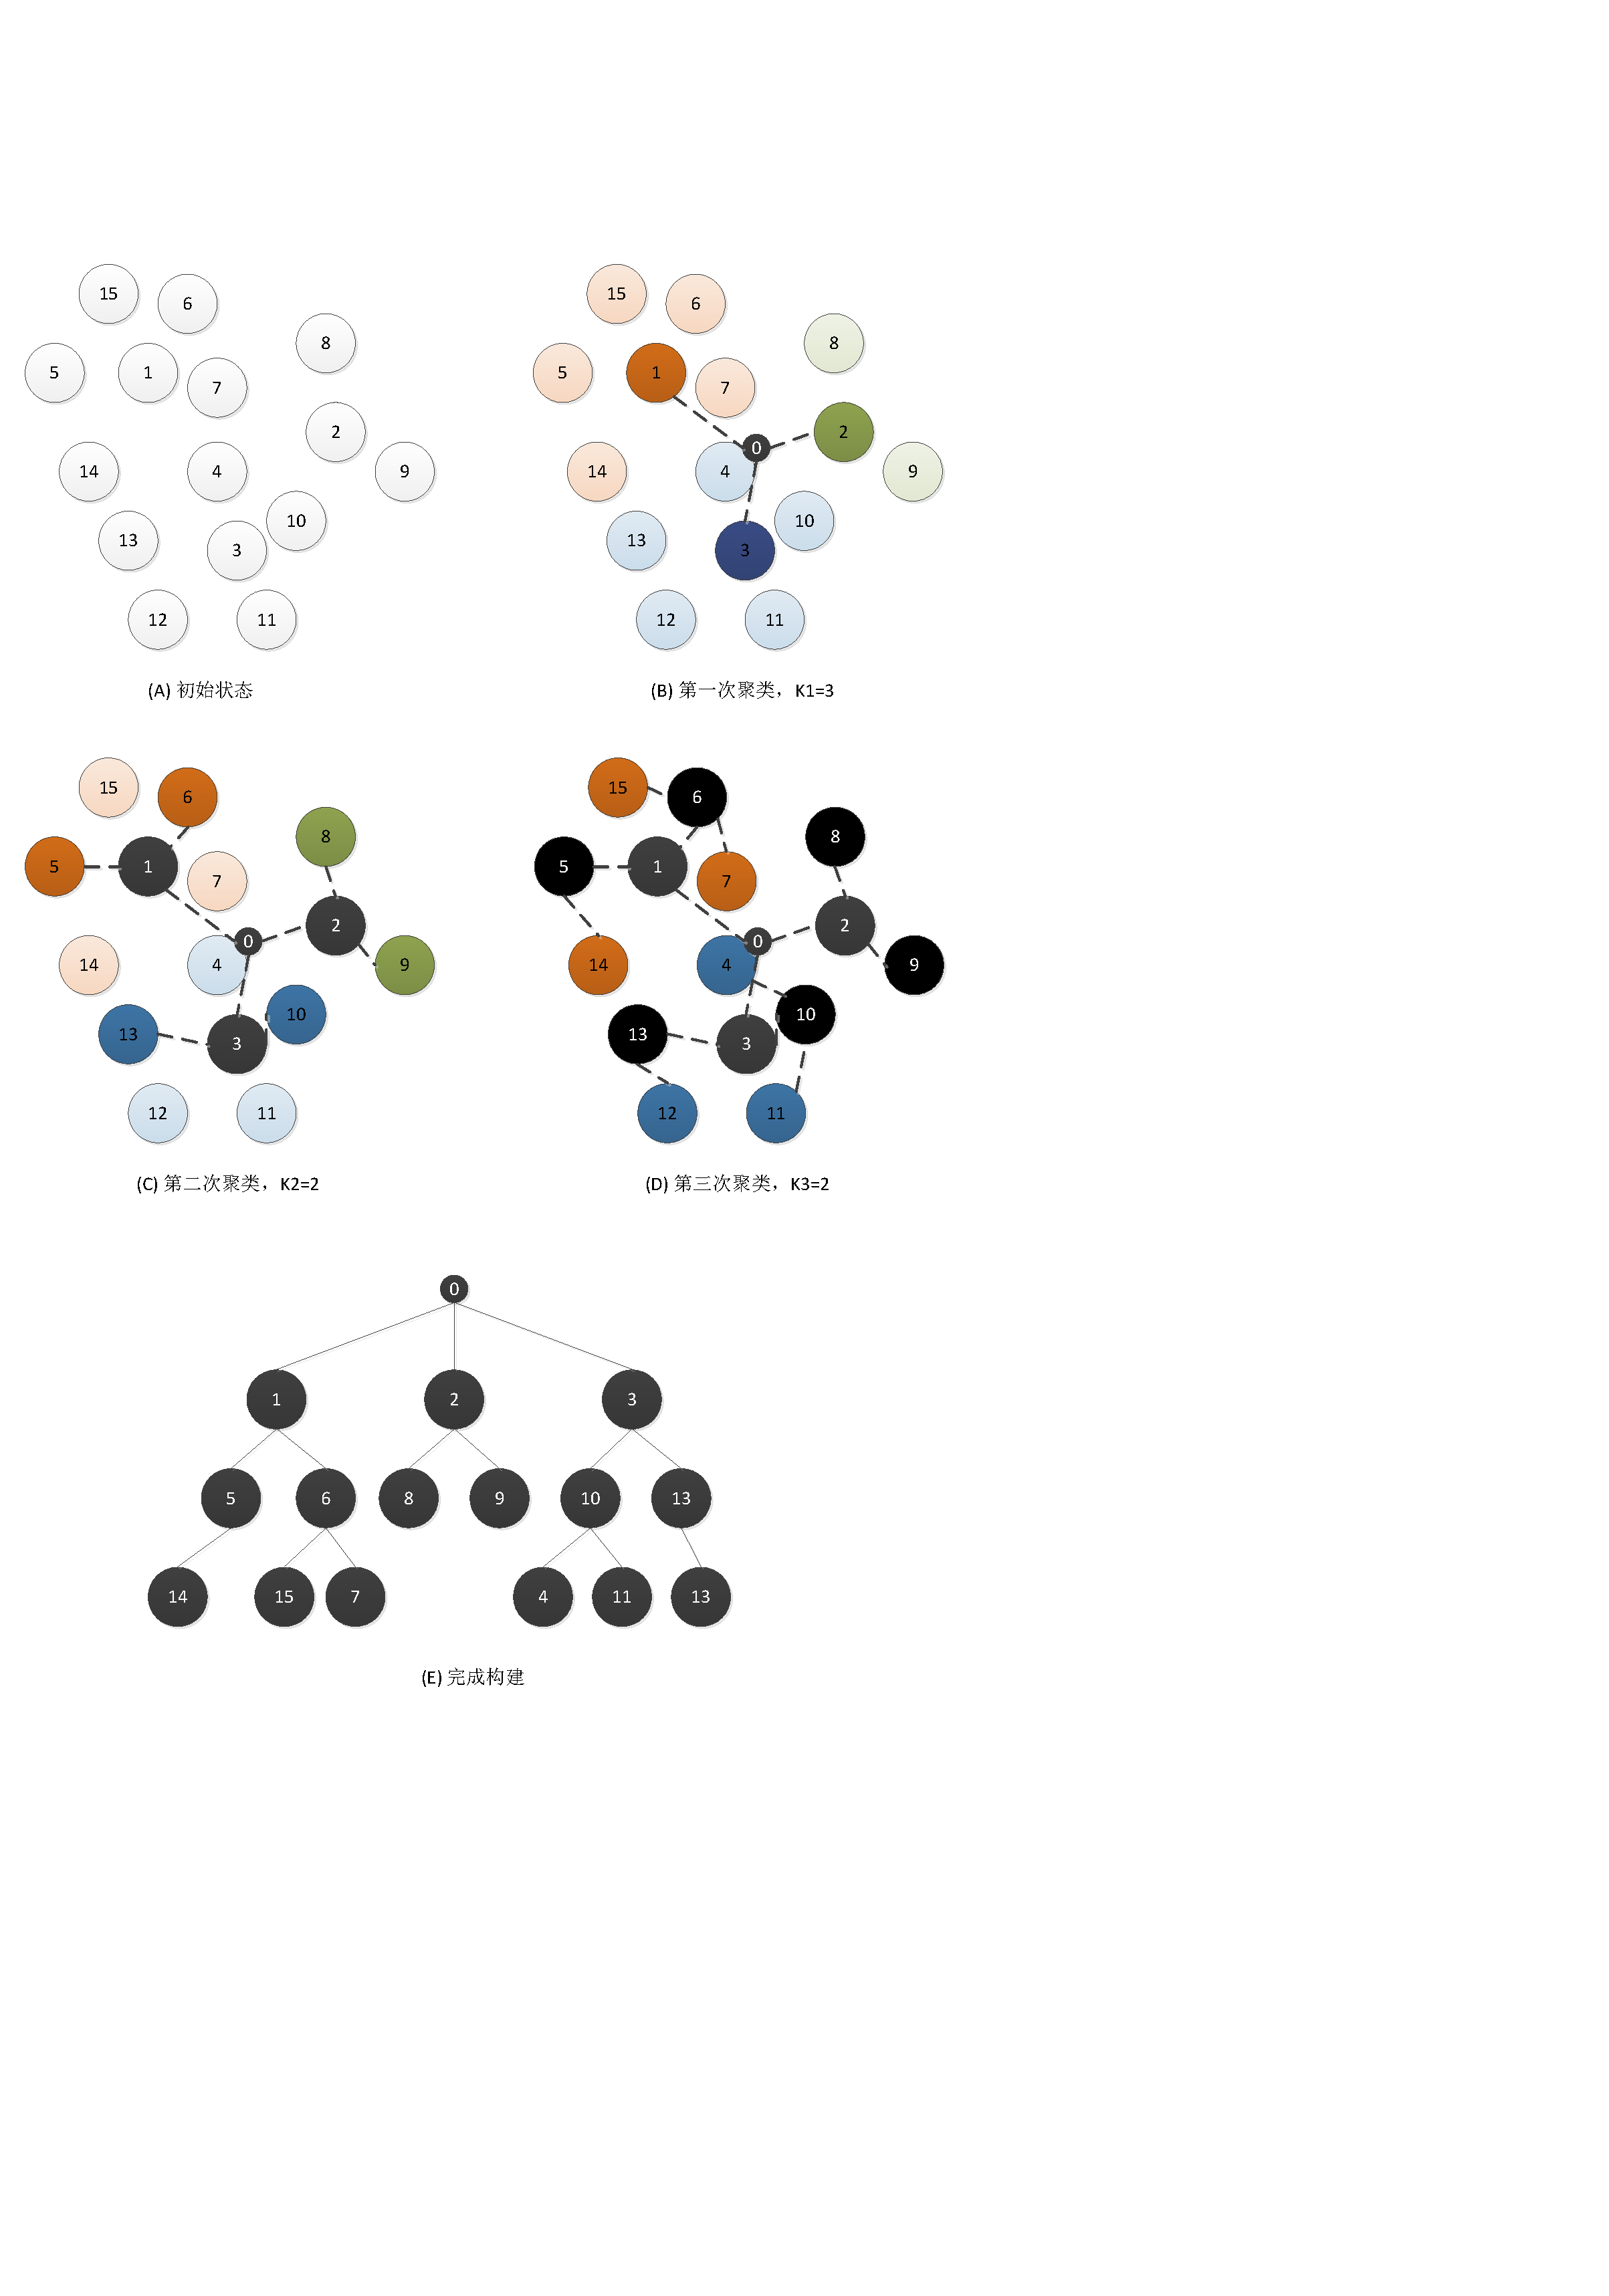
\includegraphics[width=\textwidth]{statictree.pdf}
\caption{基于兴趣余弦相似度的静态兴趣分类树的自动构建示例}
\label{fig:statictree}
\end{figure}

\subsubsection{静态兴趣分类树的构建}
在第二章中提出了几种构建静态兴趣分类树的方法,其中,人工构建法最为精确,但是对于大量的兴趣点时就会很耗时间和精力。相对的是自动构建法,其能够快速自动地对兴趣集合$\mathcal{I}$构建兴趣分类树,但是精确度是一个问题,下面来详细讨论一下基于公式\ref{eq:intsim}计算出来的兴趣相似度为何不能体现出兴趣的层次结构。

首先回顾一下自动构建兴趣分类树的方法,参照图\ref{fig:statictree}中的实例进行详解其每一步的过程:
\begin{enumerate}
  \item 对于初始化状态的兴趣点集合,它们之间可以通过公式\ref{eq:intsim}计算相似度。如图中(A)所示,初始状态一共有15个不同的兴趣点,编号从1至15。
  \item 因为根节点并不表示任何兴趣,所以虚构一个根节点0,所以第一步是构建树中的第二层。如图中(B)所示,先手动给定要聚成3类,那么根据聚类算法(这里假设是K-means)可以分成三个不同颜色的类,其中节点1、2、3分别是三个类的中心,中心的点在兴趣集合中表示该兴趣点涉及的概念和范围更加广泛,因此更适合做该类中其他节点的父节点。最后这三个中心节点与根节点相连,形成树中的第一层。
  \item 第二步是构建树中的第三层。如图中(C)所示,这是给定要在三个类中各自再聚成2类,经过聚类算法实施后,执行和第一步一样的操作。
  \item 第三步是构建树中的第四层。如图中(D)所示,这次依然给定要聚成2类,这时因为各类中的元素已经小于或等于2个,所以在聚类算法结束的时候正好把所有节点都可以连起来。
  \item 第四步对图重画,得到如图(E)中的一个兴趣分类树。由于这个树的结构需要变化的情况十分少,即插入新的兴趣点或删除旧的兴趣点的情况很少发生(至少相对于用户自己的兴趣变化来说),因此称之为静态兴趣分类树。
\end{enumerate}

从上面的过程可以看出,兴趣分类树的构建基础依赖于兴趣点的余弦相似度,树中每一层节点的确定完全依赖于聚类过程中的中心节点,而在树中父节点与孩子节点的实际意义是位于父节点的兴趣点在概念和内容上比处于孩子节点的兴趣点更加宽泛。换句话说,在这个构建的过程中,“宽泛概念”的表现是树中的层次结构,其量化的方法是对“中心节点”的求解,而中心节点的计算又依赖于余弦相似度,因此这里的假设前提是由普通的余弦相似度得到的节点间距离能够反映出层次结构。

\begin{figure}[ht]
\centering
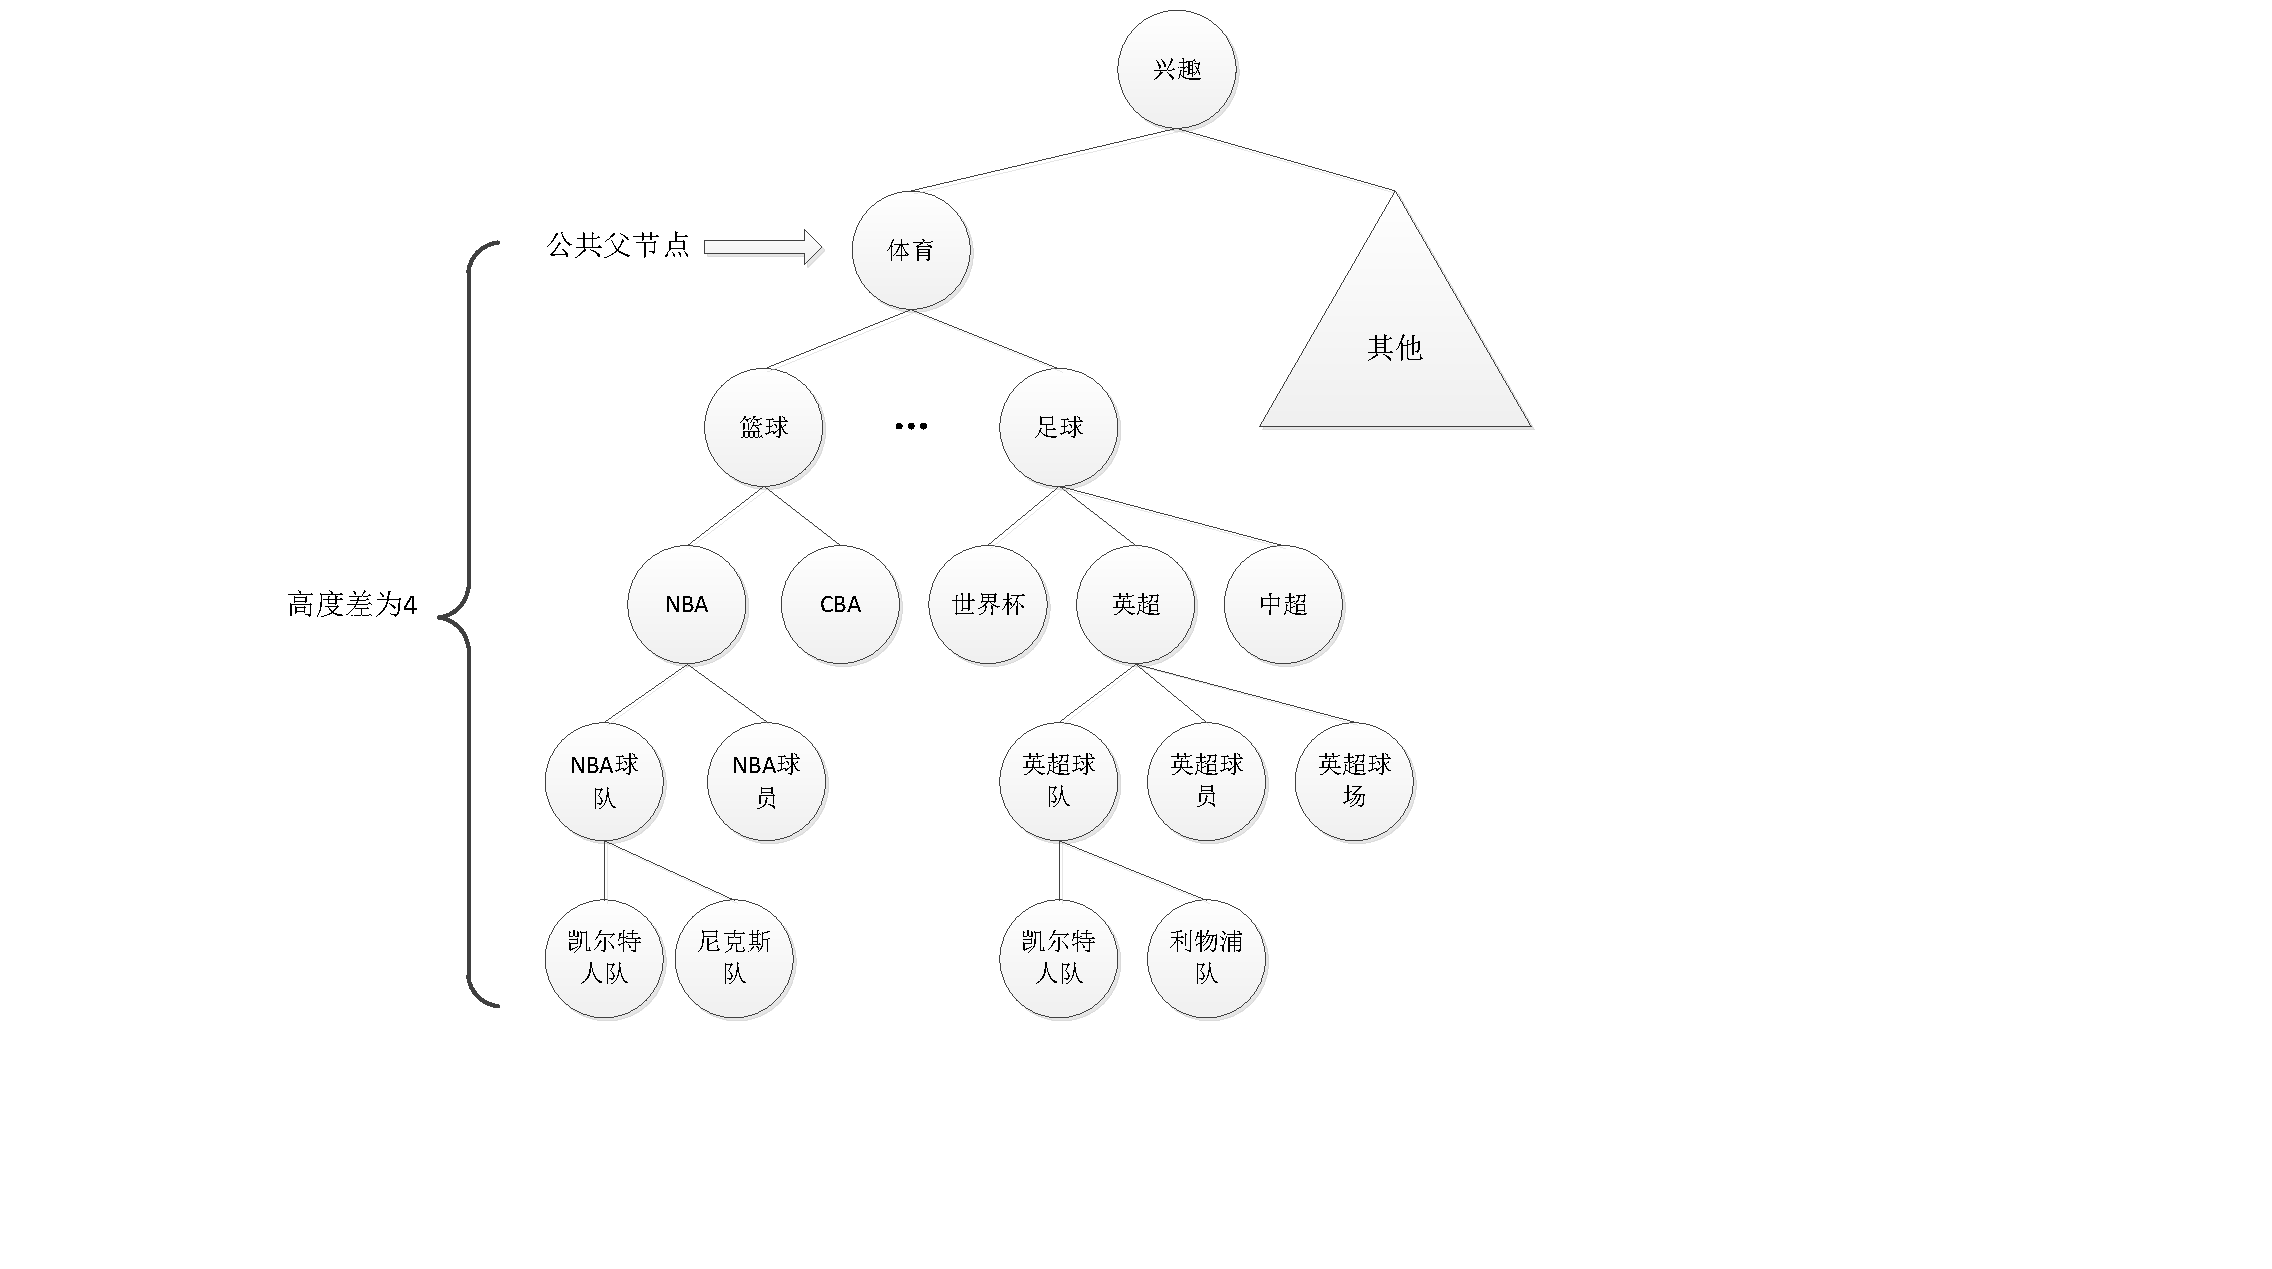
\includegraphics[width=\textwidth]{treeexample.pdf}
\caption{人工构建的一个静态兴趣分类树的实例}
\label{fig:treeexample}
\end{figure}

但是经过仔细思考之后发现,上述假设存在一定的瑕疵。举个反例来说,如图\ref{fig:treeexample}所示的是一种人工构建的可能的静态兴趣分类树。在树中的最底层分别有两个兴趣点都叫做“凯尔特人队”,但是它们一个父节点是“NBA球队”,另一个父节点是“苏超球队”,而且它们的公共父节点是“体育”,距离它们的高度分别都是4,也就是说这两个兴趣点其实差别比较大,于是,按照上述理论得出之间的余弦相似度应该比较小才对。但是事实上,这两个兴趣点的相似度会十分地接近。如表格\ref{tbl:celtics}所示,两个“凯尔特人队”的兴趣点在主题词上的相似性很大,比如“得分”、“防守”、“冠军”等词的权重都非常高。如果仅仅考虑用余弦相似度来计算两者的层次关系时,两者在层次结构上会非常地接近,因此与人工判别的实际情况矛盾。

从而可以看出,仅仅使用余弦相似度来判断兴趣点所在树中的层是存在不足的。所以在条件允许的情况下,使用人工构建的办法来建立一棵全局的静态兴趣分类树是一个更好的办法,主要是保证了层级之间兴趣点的准确性。

\begin{table}[ht]
\caption{“凯尔特人队”兴趣点的向量实例}
\centering
\begin{tabular}{cc|cc} 
\hline
“凯尔特人队(NBA)” & 权值 & “凯尔特人队(苏超)” & 权重 \\
\hline
得分 & 0.131 & 联赛 & 0.201 \\
比赛 & 0.112 & 财务 & 0.098 \\
进攻 & 0.084 & 冠军& 0.082 \\
防守 & 0.048 & 得分 & 0.065 \\
季后赛 & 0.030 & 抽签 & 0.021 \\
首轮 & 0.019 & 防守 & 0.011 \\
击败 & 0.014 & 击败 & 0.007 \\
篮球 & 0.009 & 赞助商 & 0.007 \\
伤病 & 0.003 & 点球 & 0.005 \\
冠军 & 0.001 & 赛事 & 0.002 \\
\hline
\label{tbl:celtics}
\end{tabular}
\end{table}

\subsubsection{基于静态兴趣分类树修正的兴趣点匹配}
假设根据一定的办法人工或者半自动地构建出一个全局的静态兴趣分类树后,接下来可以利用这棵树对兴趣点匹配的机制进行修正。在上一节中,已经讨论过直接通过余弦相似度计算出来的兴趣点相似度不能很好反映层级的关系,因此,可以利用已经存在的静态兴趣分类树对兴趣点的相似度在层级关系上进行修正,从而是其更加符合实际情况。

给定两个兴趣点$\vec{in}_i$和$\vec{in}_j$,可以在静态兴趣分类树中找到它们所在的层数和位置,记$h_i$为兴趣点$\vec{in}_i$在树中的高度,$H$为树的高度。通过计算还能够得到两个节点的最近公共祖先(LCA)节点$\vec{in}_p=lca(\vec{in}_i,\vec{in}_j)$。于是,定义修正过后的两个兴趣点相似度$d_{i,j}'$如下:
\begin{equation}
  d_{i,j}'=\varepsilon^{\Delta h-1}\cdot cos(\vec{in}_i,\vec{in}_j),~~(0<\varepsilon<1)
\end{equation}
其中,
\begin{equation*}
\Delta h=\frac{1}{H}\cdot max\{h_p-h_i,h_p-h_j\}
\end{equation*}

这里,$\varepsilon^{\Delta h-1}$看做是一个松弛因子,当兴趣点距离最近公共祖先节点越远时,松弛因子越小,从而相当于对原本的余弦相似度进行缩小,使其更加不相似;反之,当兴趣点距离最近公共祖先节点越近,松弛因子越大,从而余弦相似度表达得越准确。同时,当两个兴趣点具有公共父节点时,松弛因子等于1,即保持原来的余弦相似度。

\subsection{动态兴趣伸展树的表示方法}
静态兴趣分类树的作用是给全局的用户兴趣建立一个能够表示兴趣层次关系的结构,以此来更好地计算具有层次关系的用户兴趣相似度。在这一节中将考虑用户兴趣的另一个特征:动态性。参考第三章中针对文本流的主题识别问题,用户往往会在$[t_1,t_2]$时间段内产生某一个兴趣点,然后在$[t_2,t_3]$时间段内产生另一个兴趣点,现状假设已经对文本流分析出一个长度为$L$的主题序列,也即对应于长度为$L$的用户兴趣序列,记作$seq=(\vec{in}_{k_1},...,\vec{in}_{k_L}),~(k_i\in\{1...K\})$,所以,问题就转换为如何能够动态地存储和表示这种兴趣序列。

\subsubsection{动态兴趣伸展树的构建}
\begin{figure}[ht]
\centering
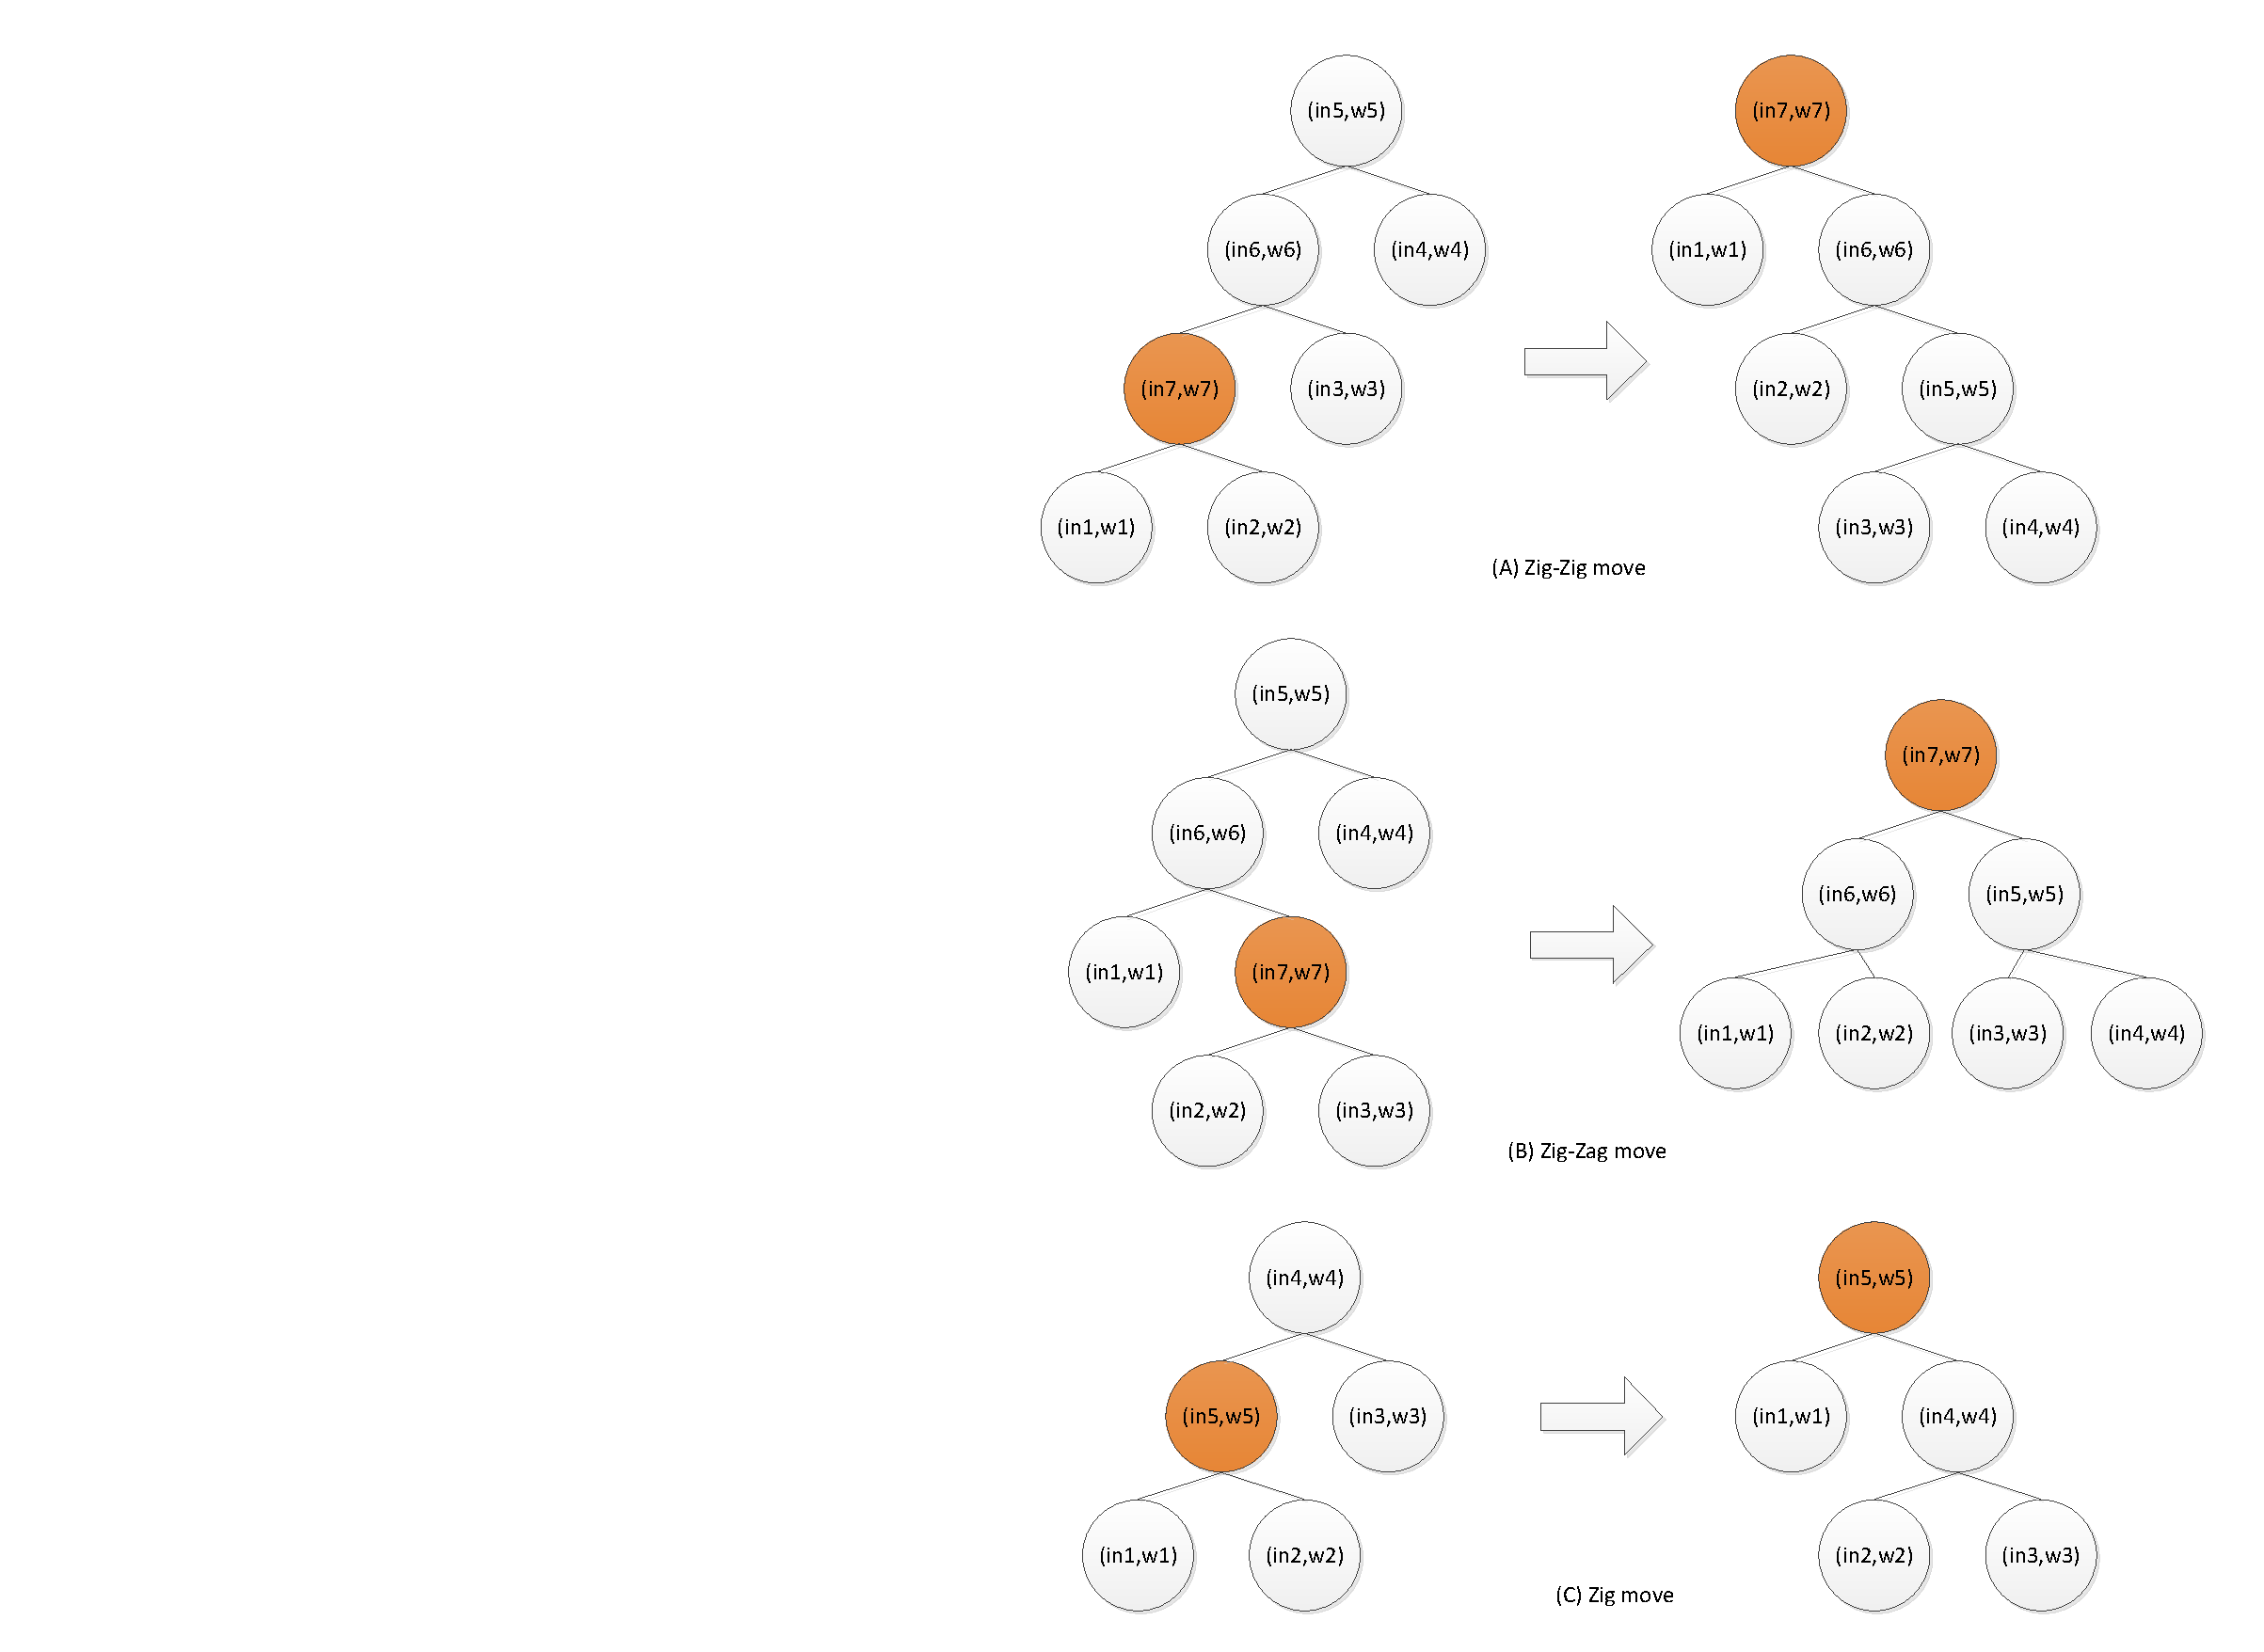
\includegraphics[width=0.9\textwidth]{zigzag.pdf}
\caption{动态兴趣伸展树在不同情况下的节点查询实例}
\label{fig:zigzag}
\end{figure}

在伸展树中,最近访问的节点总是会通过旋转进行上浮,而不经常访问的节点则会下沉。伸展树是一种平衡的二叉搜索树,在结构上,它是相同于普通二叉搜索树,唯一不同的在于算法寻找,插入和删除条目。所有伸展树操作为$O(log n)$的平均时间,其中$n$为在树中的条目的数量。任何单一的操作在最坏的情况下达到$\Theta(n)$时间。但任何对伸展树的连续操作,且树最初是空的并且从来没有超过$n$个项目的条件下,最坏情况下需要$O(K log n)$的时间。伸展树的目的是为了快速访问到那些最近刚被访问的节点,所以他们真正擅长的应用场景是大多数的查找操作的目标都是小条目。因此,这个数据结构非常适合描述用户兴趣随时间的变化。

在动态兴趣伸展树中,节点$node_i$表示第$i$个兴趣点$\vec{in}——i$,节点的键表示用户对兴趣$\vec{in}_i$的喜好程度$key(node_i)=w_i~~(w_i\in [0,1])$该值用于判断节点之间的大小关系,节点的值表示兴趣$\vec{in}_i$的兴趣分布$val(node_i)=(v_1,...,v_V)$,对应文本中的一个主题分布。当用户对某一类主题的文本发生兴趣时,等价地认为在动态兴趣伸展树中查找了对应节点。在查找过程中,树中被查找的节点会根据一系列的旋转直至最后作为根节点,如图\ref{fig:zigzag}所示为被查询节点旋转的情况。

相比较而言,在普通的二叉搜索树中执行的单个旋转,一些节点在树中移动高,一些较低。在左旋转时,父节点向下移动,其右子节点上移一个层。在双旋转时,是由两个单转组成,并且一个节点向上移动两个层,而所有其他的向上或向下移动通过至多一个层。从刚刚访问的目标节点开始向上移动直至根节点,可以在每一步做单一旋转,从而把该节点一路升至根。这种方法将实现使目标节点到根的目标,但是,事实证明,分摊在很多访问树的性能可能不太好。相反,伸展的关键思想是在每一步中将目标节点向上移动两层。考虑从根下降到刚访问节点的路径,每一次向左下移动时,称之为zig,而每次向右下移动,则称之为zag。向左下移动两步称为zig-zig,右下两步称为zag-zag,先左再右称为zig-zag,先右后左称为zag-zig。这四种情况在移动两步下来的路径中存在唯一的可能。但是如果路径的长度为奇数,最后将多一个步骤,即zig或者zag中的一步。

\begin{figure}[ht]
\centering
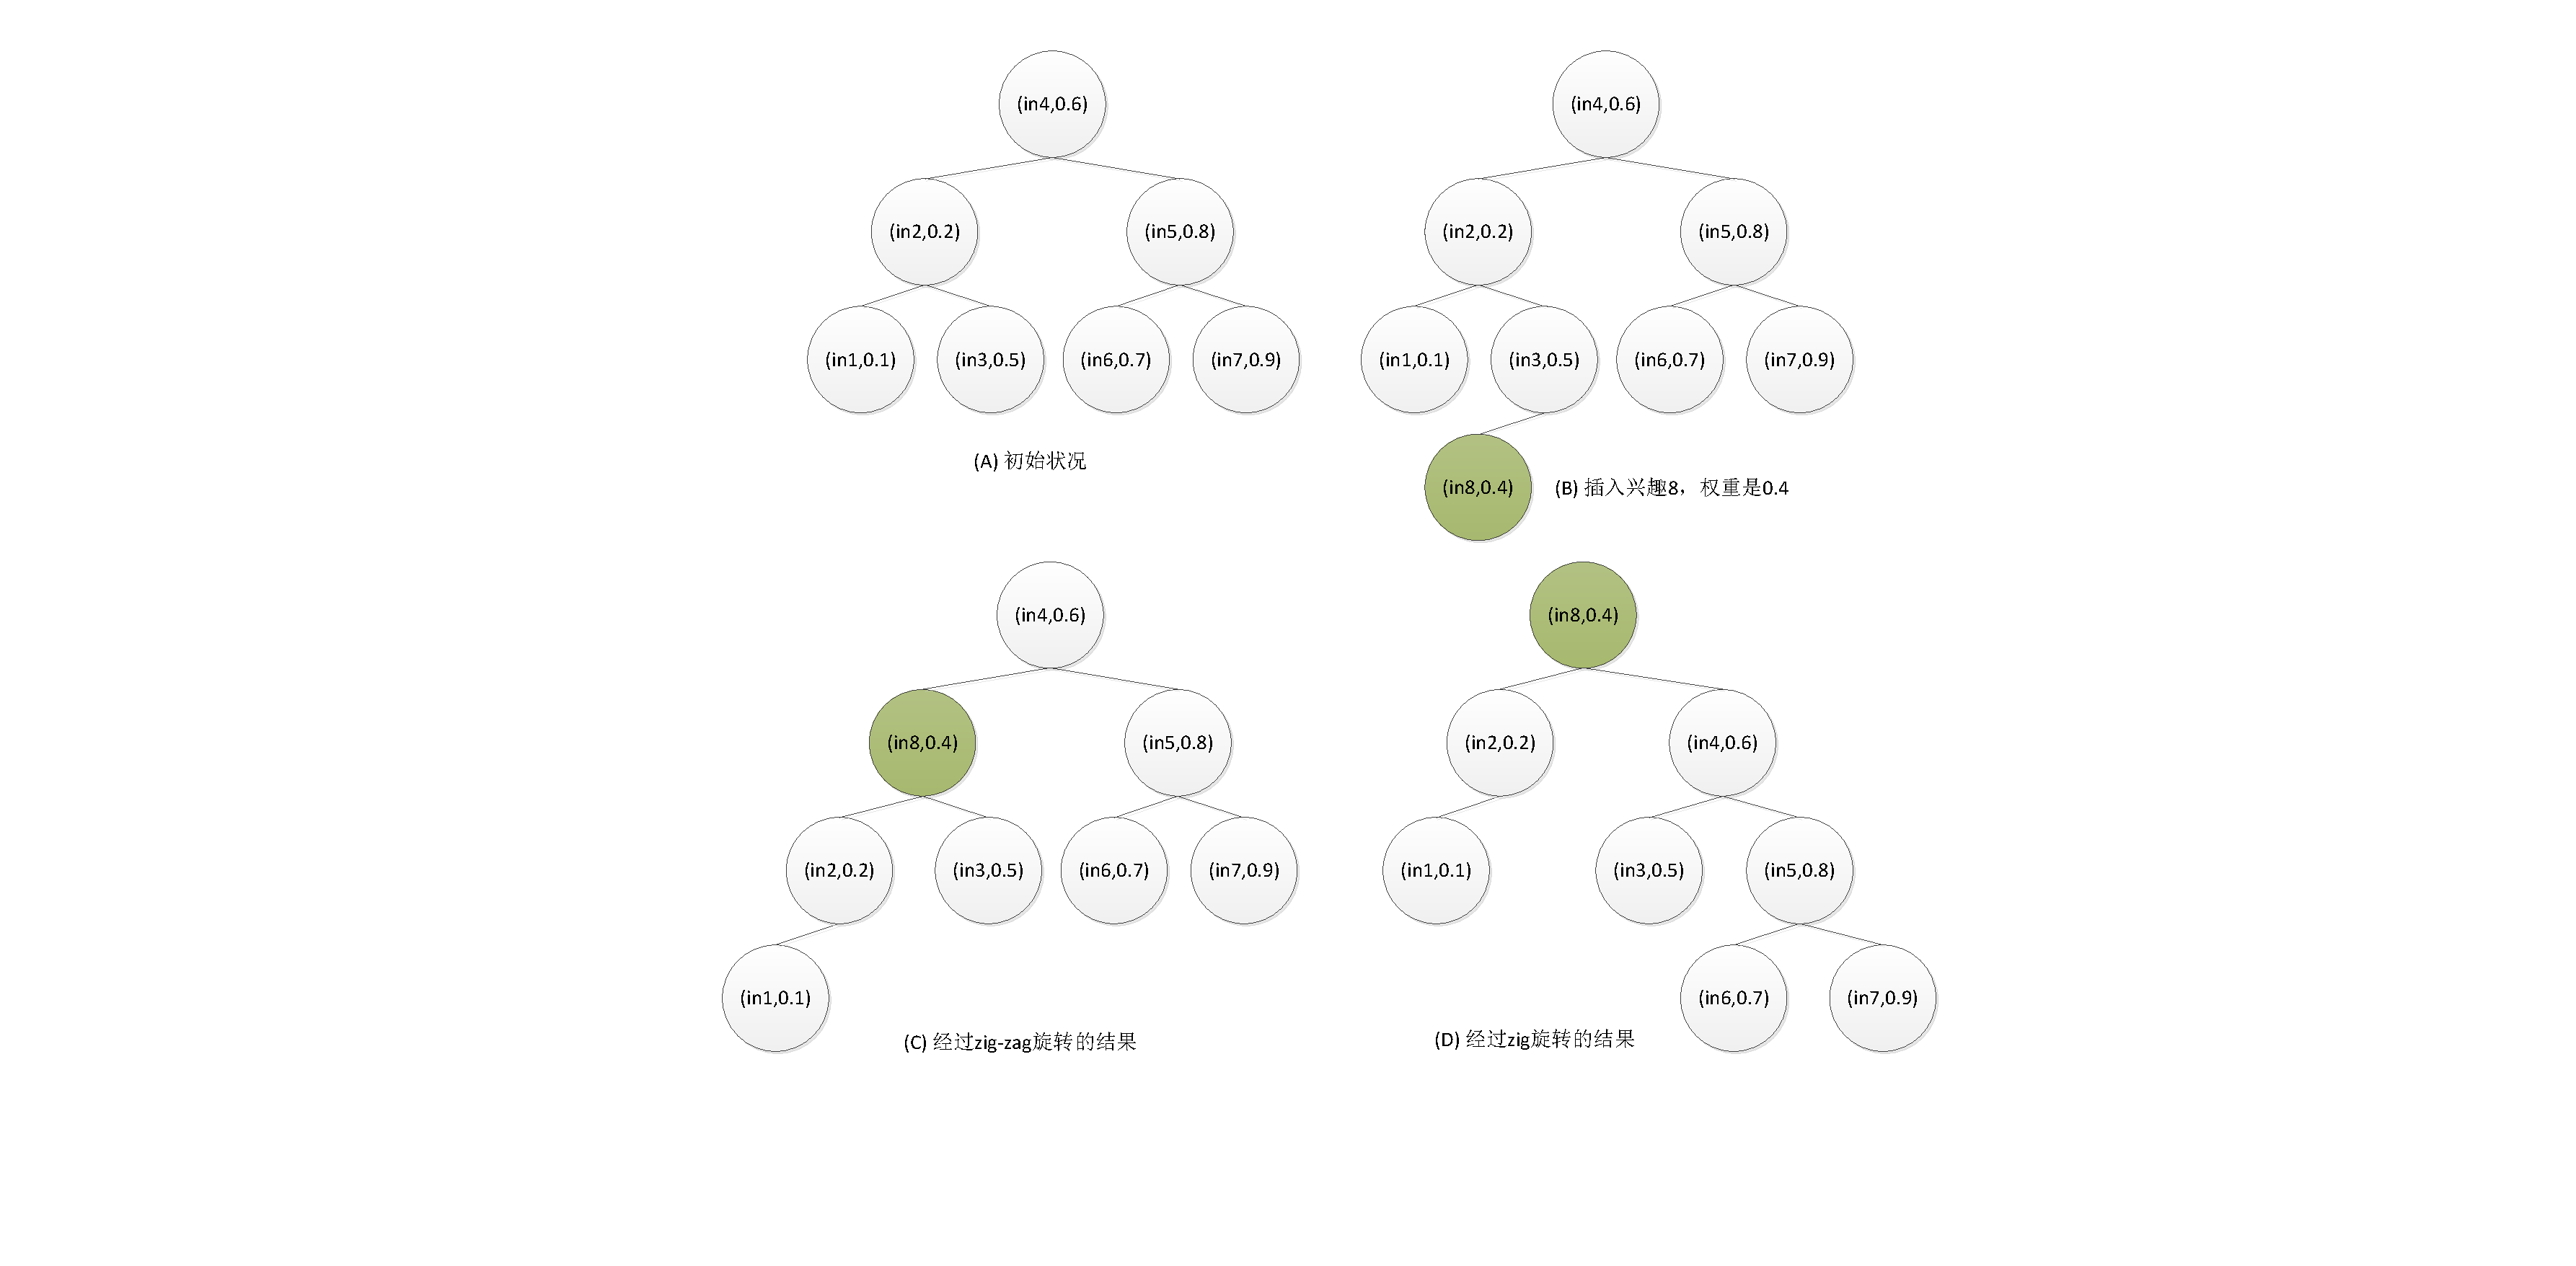
\includegraphics[width=\textwidth]{splayinsert.pdf}
\caption{动态兴趣伸展树添加兴趣点的实例}
\label{fig:splayinsert}
\end{figure}

当用户产生新的兴趣时,则需要对动态兴趣伸展树进行插入节点的操作,如图\ref{fig:splayinsert}所示。图(A)中表示用户在某一时刻下动态兴趣伸展树的初始状态,每个节点中$(in,w)$表示(兴趣编号,权重),这里省略了兴趣分布。在图(B)中,现在要插入一个新的兴趣8,其权重为4,于是先从根节点开始搜索,找到改新增节点在二叉搜索树中的位置,接下来的任务是把该节点向上移动到根节点处。图(C)中展示了在经过一次zig-zag旋转之后,兴趣8节点所在的位置。最后,再经过一次zig旋转,将兴趣8节点上移至了根节点出,最后的动态兴趣伸展树的结构如图(D)所示。

关于在动态兴趣伸展树上的其他操作,比如删除节点,合并两个兴趣伸展树等等,将不再详细说明,具体的方法与上述思想类似。

\subsubsection{基于动态兴趣伸展树修正的兴趣点匹配}
动态兴趣伸展树其实表示的是用户在某一时段内兴趣的变化状态,而普通的通过兴趣向量计算出的两个用户之间的兴趣相似度则体现不出这一点,因此可以利用动态兴趣伸展树对其进行一定程度上的修正。

对于用户兴趣向量$D=\{(i_1,w_1),...,(i_K,w_K)\}$,其中$i_1,...,i_K$表示$K$个兴趣的编号,$w_1,...,w_K$表示用户对$K$个兴趣的喜好程度,简单来说就是权重,其值的范围是$[0,1]$。兴趣向量的求解方式可以是通过对用户涉及的所有历史文档进行主题分析,不同类型的文档主题识别方式已经在上一章详细讨论。可以看出,这种兴趣向量是一种比较全局的描述,因此无法体现出用户近期的兴趣程度。而利用动态兴趣伸展树的结构可以弥补这个兴趣向量在动态性上的不足。于是,定义修正后的兴趣$i_k$的权重$w_k'$为:
\begin{equation}
  w_k'=\varepsilon^{h-1}\cdot w_k,~~(0<\varepsilon<1)
\end{equation}
其中,$h$表示兴趣$i_k$对应节点在动态兴趣伸展树中的深度,$\varepsilon^{h-1}$是一个松弛因子。

当兴趣节点距离根节点越远时,松弛因子越小,说明这个兴趣节点很少被访问,即用户已经很久没有对这个兴趣有喜好了;相反,当兴趣节点距离根节点越近时,松弛因子越大,说明这个兴趣节点最近刚刚被访问过,也即用户最近看过具有对应主题的文章了;当兴趣节点是根节点时,松弛因子是1,即兴趣权重没有变化。

同时,当原有的$w_k$很大时,该兴趣是一个长期兴趣,反之是一个短期兴趣,长期兴趣即使乘以一个较小的松弛因子时,其权重相对于其他短期兴趣的权重来说还是很大的,所以该方法同时保证了用户的长期兴趣和短期兴趣。

\subsection{基于用户兴趣树的自动推荐方法}
在这一节中,

\subsection{小结}
在这一章中,提出了两种兴趣树的结构用来充分体现用户兴趣的特征。静态兴趣分类树反映的是用户兴趣之间的层次关联性。在计算两个兴趣点的相似度时,如果仅仅对兴趣对应的主题分布求余弦相似度的话并不能体现出兴趣点之间的层次性,因此需要利用静态兴趣分类树对这个相似度进行修正。类似的,动态兴趣伸展树反映的是用户兴趣随时间变化的动态性。在计算用户的兴趣向量时,由于每个兴趣点对应的权值反映的是全局用户兴趣的特征,因此不能反映最新实时的用户兴趣,所以需要利用动态兴趣伸展树对这个权重进行修正。
